So far, this paper has introduced various recommendation techniques and metrics implemented in \texttt{Recommendation.jl}. This section finally evaluates the recommenders on different metrics. Since the purpose of the following experiment is to demonstrate the capability of \texttt{Recommendation.jl} and undergo trade-off discussions among different metrics, we test only on the minimal MovieLens 100k dataset \cite{harper2015movielens} and use the \texttt{SVD} recommender (\sect{svd}) as a model-based advanced option, which requires the simplest set of hyperparameters, along with multiple baselines. However, developers can easily evaluate larger datasets with more complex models in the same way as we describe below.

We conducted a 5-fold cross-validation of top-10 recommendations on the 100,000 user-item-rating pairs, by randomly splitting the data into five distinct sets. For each trial, we call \texttt{fit!()} on four-fifths of them (80\% samples) and then run top-10 \texttt{recommend()} for every user. Ultimately, resulting recommendations, as well as predicted ratings, are compared with the ones observed in the rest of 20\% samples for validation.\footnote{A complete Julia script used for the experiment can be found at \url{https://github.com/takuti/Recommendation.jl/blob/v1.0.0/examples/benchmark.jl}.}

\begin{lstlisting}[language = Julia]
n_folds = 5
topk = 10
data = load_movielens_100k()
cross_validation(
    n_folds, metrics, recommender, data,
    params...)
\end{lstlisting}

\tab{results} summarizes the results obtained from each recommender-metric pair. On the one hand, model-based SVD recommenders showed higher accuracy than the baselines in terms of both rating and ranking metrics. In particular, as the accuracy changes by $k$ for $\mathrm{SVD}_k$, we see $k = 16$ can be an optimal hyperparameter for the recommender. On the other hand, aggregated and intra-list metrics do not yield the same conclusion; since larger $k$ gives a closer approximation to real-world diverse user-item behaviors, $\mathrm{SVD}_{32}$ shows the highest aggregated diversity and Shannon entropy. These observations demonstrate the trade-off between accuracy and non-accuracy metrics as \fig{tradeoff} depicts.

\begin{figure}[htbp]
    \centering
    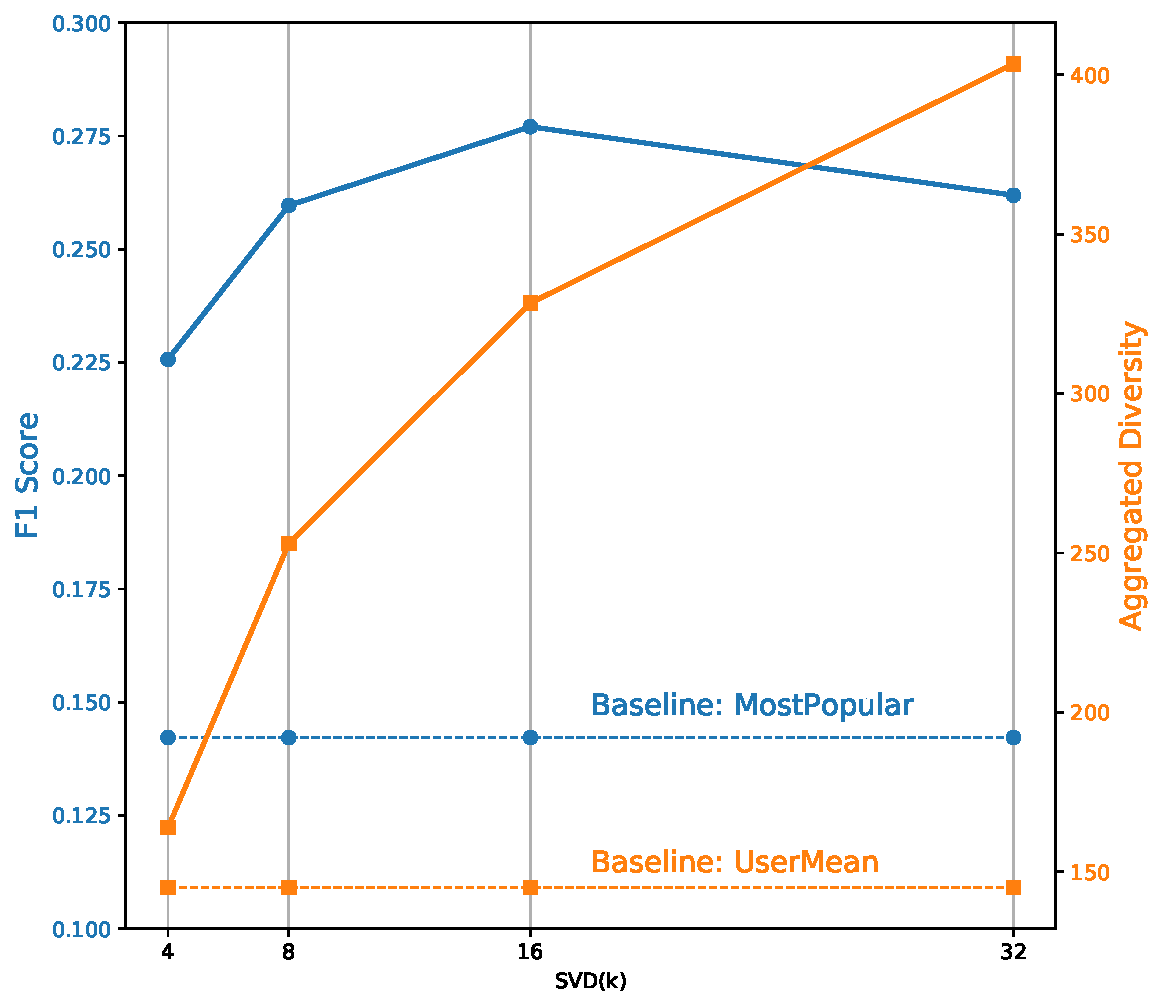
\includegraphics[width=1.0\linewidth]{images/tradeoff.pdf}
    \caption{$F_1$ score (accuracy metric calculated by $2 \frac{\mathrm{recall} \cdot \mathrm{precision}}{\mathrm{recall} + \mathrm{precision}}$) and aggregated diversity (non-accuracy metric) for $\mathrm{SVD}_k$ recommenders, based on the numbers in \tab{results}. The accuracy graph shows that an optimal $k$ is $16$ where $F_1$ score is maximized, whereas diversity monotonically increases as $k$ gets larger. Best baseline metrics are illustrated as dashed lines for reference.}
    \label{fig:tradeoff}
\end{figure}

\begin{table*}[]
    \centering
    \tbl{Results from 5-fold cross-validation of top-10 recommendation conducted on MovieLens 100k user-item-rating pairs. Numbers are rounded to 3 decimal places, and those in the bold font indicate the ``best'' values for each metric. Accuracy metrics for \texttt{MostPopular} are not calculated because the recommender does not explicitly predict ratings.}{
    \begin{tabular}{|cl||r|r|r|r|r|r|r|}
    \hline
    \multicolumn{2}{|c||}{}                                                                                                           & \texttt{ItemMean} & \texttt{UserMean} & \texttt{MostPopular} & \texttt{SVD(4)} & \texttt{SVD(8)} & \texttt{SVD(16)} & \texttt{SVD(32)} \\ \hline \hline
    \multicolumn{1}{|c|}{\multirow{2}{*}{\begin{tabular}[c]{@{}c@{}}Rating\\ (\sect{rating-metrics})\end{tabular}}}         & \texttt{RMSE               } & 0.642    & 0.681    & -           & 0.545  & \textbf{0.524}  & \textbf{0.524}   & 0.550   \\ \cline{2-9} 
    \multicolumn{1}{|c|}{}                                                                                           & \texttt{MAE                } & 0.603    & 0.642    & -           & 0.493  & 0.471  & \textbf{0.470}   & 0.496   \\ \hline \hline
    \multicolumn{1}{|c|}{\multirow{6}{*}{\begin{tabular}[c]{@{}c@{}}Ranking\\ (\sect{ranking-metrics})\end{tabular}}}       & \texttt{Recall             } & 0.108    & 0.002    & 0.114       & 0.182  & 0.212  & \textbf{0.228}   & 0.218   \\ \cline{2-9} 
    \multicolumn{1}{|c|}{}                                                                                           & \texttt{Precision          } & 0.185    & 0.004    & 0.189       & 0.297  & 0.335  & \textbf{0.353}   & 0.328   \\ \cline{2-9} 
    \multicolumn{1}{|c|}{}                                                                                           & \texttt{AUC                } & 0.417    & 0.018    & 0.429       & 0.531  & 0.558  & \textbf{0.579}   & 0.571   \\ \cline{2-9} 
    \multicolumn{1}{|c|}{}                                                                                           & \texttt{ReciprocalRank     } & 0.415    & 0.011    & 0.409       & 0.583  & 0.642  & \textbf{0.670}   & 0.645   \\ \cline{2-9} 
    \multicolumn{1}{|c|}{}                                                                                           & \texttt{MPR                } & 84.671   & 89.784   & 84.021      & 80.192 & 78.431 & \textbf{77.417}  & 78.023  \\ \cline{2-9} 
    \multicolumn{1}{|c|}{}                                                                                           & \texttt{NDCG               } & 0.201    & 0.004    & 0.203       & 0.327  & 0.371  & \textbf{0.392}   & 0.365   \\ \hline \hline
    \multicolumn{1}{|c|}{\multirow{3}{*}{\begin{tabular}[c]{@{}c@{}}Aggregated\\ (\sect{aggregated-metrics})\end{tabular}}} & \texttt{AggregatedDiversity} & 52.2     & 145.0    & 52.4        & 163.8  & 253.0  & 328.4   & \textbf{403.4}   \\ \cline{2-9} 
    \multicolumn{1}{|c|}{}                                                                                           & \texttt{ShannonEntropy     } & 3.149    & 4.170    & 3.160       & 4.486  & 4.847  & 5.138   & \textbf{5.386}   \\ \cline{2-9} 
    \multicolumn{1}{|c|}{}                                                                                           & \texttt{GiniIndex          } & 0.662    & 0.669    & 0.658       & 0.597  & 0.629  & 0.616   & \textbf{0.599}   \\ \hline \hline
    \multicolumn{1}{|c|}{\multirow{2}{*}{\begin{tabular}[c]{@{}c@{}}Intra-list\\ (\sect{intra-list-metrics})\end{tabular}}} & \texttt{Coverage           } & 0.006    & 0.006    & 0.006       & 0.006  & 0.006  & 0.006   & 0.006   \\ \cline{2-9} 
    \multicolumn{1}{|c|}{}                                                                                           & \texttt{Novelty            } & 8.998    & \textbf{9.944}    & 8.970       & 8.763  & 8.751  & 8.991   & 9.424   \\ \hline
    \end{tabular}
    }
    \label{tab:results}
\end{table*}

Meanwhile, rule-based \texttt{UserMean} recommender, which simply scores items by a mean rating per user, was the best in terms of novelty, demonstrating the higher ability to surface unseen items at the top. In combination with the trade-off discussion above, the results tell us that focusing only on a single metric can easily confuse developers and mislead the users of recommender systems. Therefore, it is crucial to holistically assess the systems from multiple perspectives, and the design principle of \texttt{Recommendation.jl} follows the point as we explained in \sect{introduction}.

It should be noticed that, as \texttt{kwargs...} in \sect{intra-list-metrics} indicate, evaluation in intra-list metrics is not straightforward due to the need for specifying additional arguments to set up a scenario. For the sake of simplicity, this section assumes \texttt{catalog} for \texttt{Coverage} is a set of all items available in the dataset, and \texttt{observed} for \texttt{Novelty} is a set of items in target user's training samples, allowing the recommenders to recommend the same items in a training set to the same user. Thus, \texttt{Coverage} in \tab{results} is the same across the recommenders because we always recommend 10 items per user from the fixed set of all items. Moreover, we did not evaluate in \texttt{IntraListSimilarity} and \texttt{Serendipity} because there is no obvious way to define item-item similarities, relevance, and unexpectedness; the choices depend largely on the developer's hypotheses and objectives that this paper does not discuss in detail.
